\begin{problem}{Ayman and Stairs (Easy Version)}{standard input}{standard output}{2 seconds}{256 megabytes}

\textbf{The only difference between the two versions of the problem is the constraints on $n$. In this version $n \leq 10^8$.}

Ayman likes stairs very much, and does not get tired of making them. His dad brought him $n$ cubes and Ayman wonders what is the maximum length of stairs he can make with them. Can you help him to find that answer?

A sequence of stairs of length $k$ is a succession of $k$ columns made of cubes, where the $1$-st column has $1$ cube, the $2$-nd column has $2$... and so forth until the $k$-th column.

\begin{center}
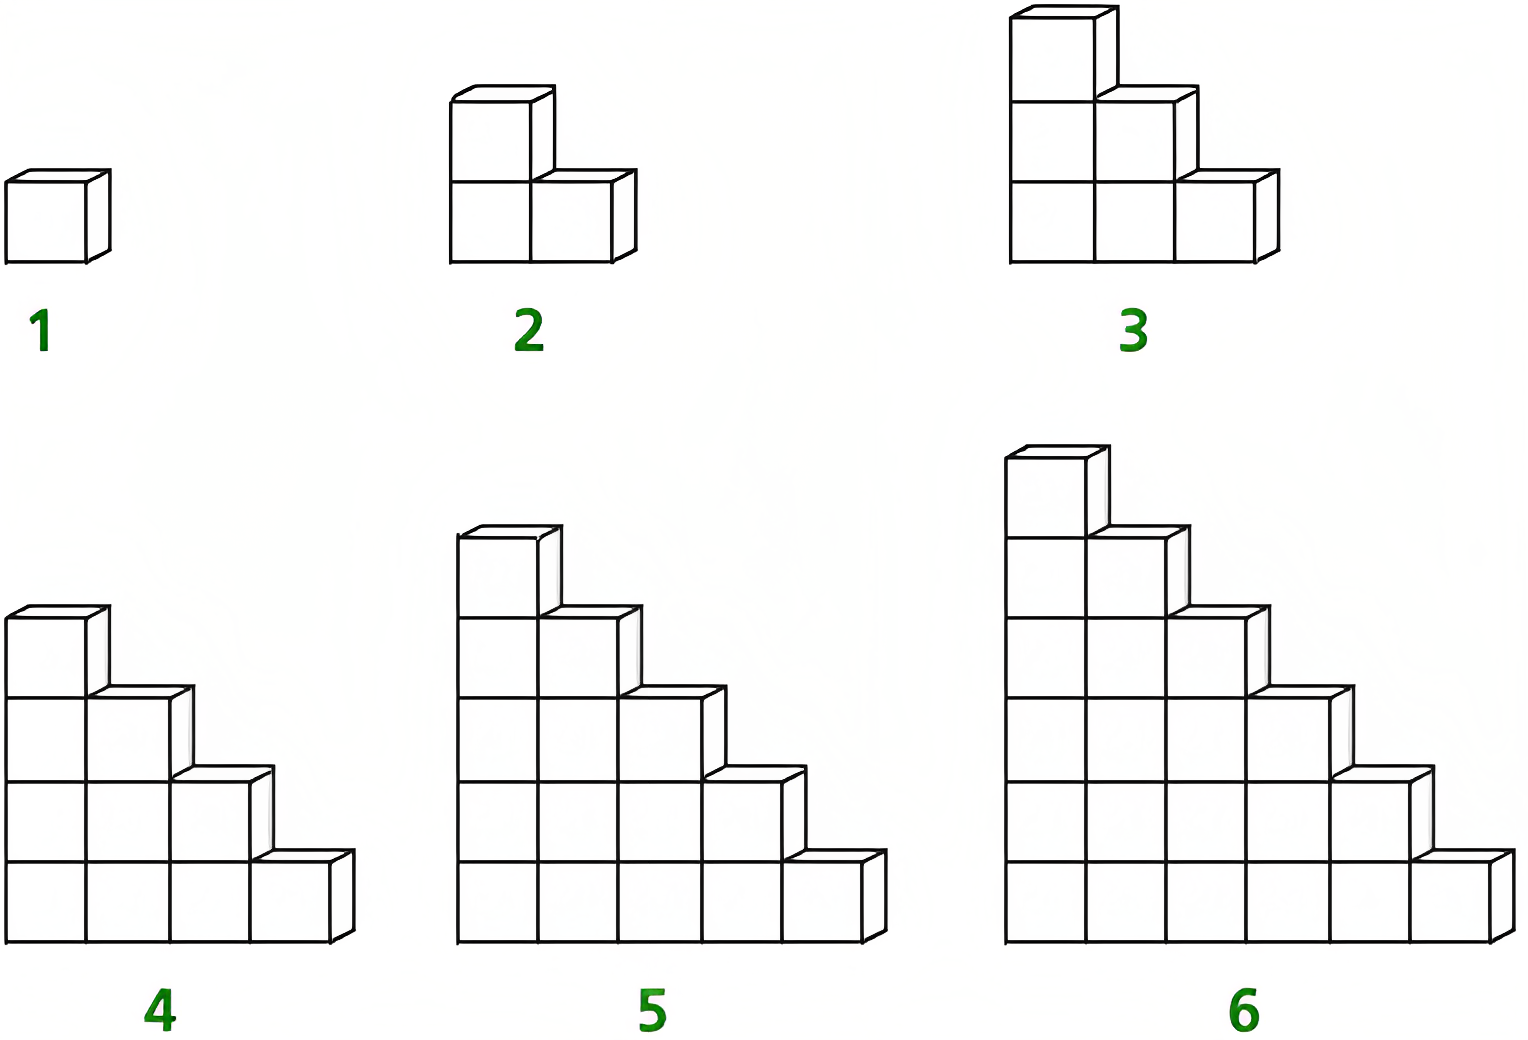
\includegraphics[width=16cm]{figure-1_2.png}
\small{Here is an example of sequences of stairs of lengths from $1$ to $6$}
\end{center}

Note that he does not have to use all the $n$ cubes.

\InputFile
A positive integer $n$ $(1 \leq n \leq 10^8)$ representing the number of cubes.

\OutputFile
Output one integer, the maximum length of stairs Ayman can make.

\Examples

\begin{example}
\exmpfile{example.01}{example.01.a}%
\exmpfile{example.02}{example.02.a}%
\end{example}

\Note
In the first testcase, he can make stairs of length $4$ with $10$ cubes.

In the second testcase, he can make stairs of length $3$ with $6$ cubes, and the remaining $2$  cubes are useless since he needs $4$ cubes to make another column.

\end{problem}

